\begin{figure}[h] 
\centering 
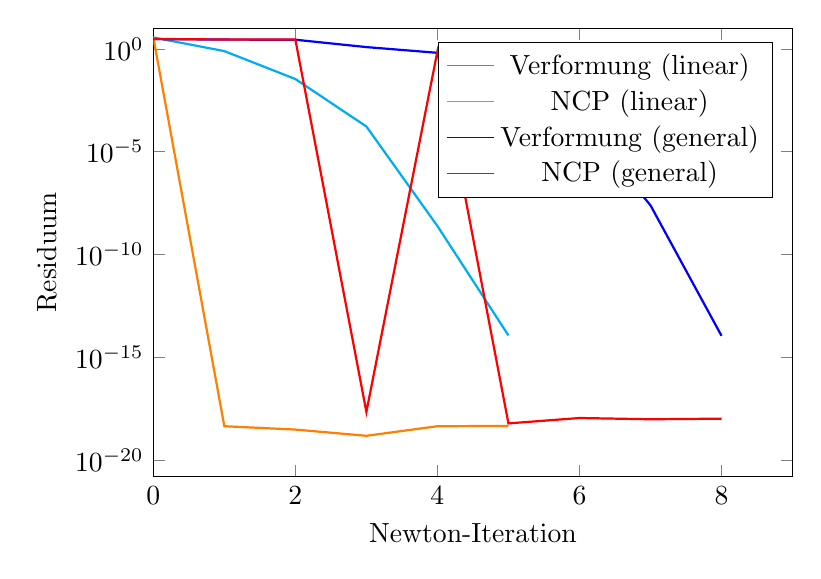
\begin{tikzpicture}[every plot/.append style={thick}] 
\begin{axis}[ 
label style={font=\normalsize}, 
xlabel={Newton-Iteration}, 
ylabel={Residuum}, 
xmin=0, xmax=9, 
ymode=log, 
ymin=0, ymax=10, 
width=0.8\textwidth, 
height=0.6\textwidth, 
legend pos=north east, 
legend style={cells={align=left}}, 
grid style=dashed, 
] 
\addplot[ 
color=cyan, 
] 
coordinates { 
(0, 3.55e+00)(1, 7.72e-01)(2, 3.39e-02)(3, 1.67e-04)(4, 2.42e-09)(5, 1.16e-14)}; 
\addlegendentry{Verformung (linear)} 
\addplot[ 
color=orange, 
] 
coordinates { 
(0, 3.64e+00)(1, 4.47e-19)(2, 3.07e-19)(3, 1.53e-19)(4, 4.47e-19)(5, 4.60e-19)}; 
\addlegendentry{NCP (linear)} 
\addplot[ 
color=blue, 
] 
coordinates { 
(0, 2.97e+00)(1, 2.80e+00)(2, 2.76e+00)(3, 1.21e+00)(4, 6.37e-01)(5, 4.94e-02)(6, 3.80e-04)(7, 2.45e-08)(8, 1.11e-14)}; 
\addlegendentry{Verformung (general)} 
\addplot[ 
color=red, 
] 
coordinates { 
(0, 3.02e+00)(1, 2.83e+00)(2, 2.81e+00)(3, 2.22e-18)(4, 7.52e-01)(5, 6.13e-19)(6, 1.12e-18)(7, 9.74e-19)(8, 1.04e-18)}; 
\addlegendentry{NCP (general)} 
\end{axis} 
\end{tikzpicture} 
\caption{Residuen des Stoffgesetzes 'Neo Hooke' mit Hinderniss 'Hut' und 578 Freiheitsgraden für die Verschiebung.} 
\label{fiq:NeoHooke_Hut_level3} 
\end{figure} 
